% Copyright 2004 by Till Tantau <tantau@users.sourceforge.net>.
%
% In principle, this file can be redistributed and/or modified under
% the terms of the GNU Public License, version 2.
%
% However, this file is supposed to be a template to be modified
% for your own needs. For this reason, if you use this file as a
% template and not specifically distribute it as part of a another
% package/program, I grant the extra permission to freely copy and
% modify this file as you see fit and even to delete this copyright
% notice. 

\documentclass{beamer}

% There are many different themes available for Beamer. A comprehensive
% list with examples is given here:
% http://deic.uab.es/~iblanes/beamer_gallery/index_by_theme.html
% You can uncomment the themes below if you would like to use a different
% one:
%\usetheme{AnnArbor}
%\usetheme{Antibes}
%\usetheme{Bergen}
%\usetheme{Berkeley}
%\usetheme{Berlin}
%\usetheme{Boadilla}
%\usetheme{boxes}
%\usetheme{CambridgeUS}
%\usetheme{Copenhagen}
%\usetheme{Darmstadt}
%\usetheme{default}
%\usetheme{Frankfurt}
%\usetheme{Goettingen}
%\usetheme{Hannover}
%\usetheme{Ilmenau}
%\usetheme{JuanLesPins}
%\usetheme{Luebeck}
\usetheme{Madrid}
%\usetheme{Malmoe}
%\usetheme{Marburg}
%\usetheme{Montpellier}
%\usetheme{PaloAlto}
%\usetheme{Pittsburgh}
%\usetheme{Rochester}
%\usetheme{Singapore}
%\usetheme{Szeged}
%\usetheme{Warsaw}
\usepackage{xcolor}
\setbeamercovered{transparent}
\usepackage{amsmath}
\usepackage{eucal}
\usepackage{graphics}
\usepackage[justification=centering]{caption}

\defbeamertemplate*{footline}{mytheme}
{
    \leavevmode%
          \hbox{%
              \begin{beamercolorbox}[wd=.3\paperwidth,ht=2.25ex,dp=1ex,center]{section in head/foot}%
                  \usebeamerfont{author in head/foot}~{Mohammed~Khatiri}
              \end{beamercolorbox}%
              \begin{beamercolorbox}[wd=.4\paperwidth,ht=2.25ex,dp=1ex,center]{section in head/foot}%
                  \usebeamerfont{author in head/foot}~\insertshorttitle{}
              \end{beamercolorbox}%
              \begin{beamercolorbox}[wd=.3\paperwidth,ht=2.25ex,dp=1ex,right]{section in head/foot}%
                  \usebeamerfont{date in head/foot}
                  \insertframenumber{} / \inserttotalframenumber\hspace*{2ex} 
              \end{beamercolorbox}}%
                  \vskip0pt%
              }
\usebeamertemplate{mytheme}



\title{Les architectures Microservices}

% A subtitle is optional and this may be deleted
\subtitle{id\'ee g\'en\'erale et avantages}

\author{Mohammed~Khatiri\inst{2}\inst{1}}
% - Give the names in the same order as the appear in the paper.
% - Use the \inst{?} command only if the authors have different
%   affiliation.

\institute[Univ. Grenoble Alpes, CNRS, Inria, LIG] % (optional, but mostly needed)
{
    \inst{1}%
  University Mohammed First\\
  Faculty of Sciences, LaRI, Morocco\\
  \textcolor{red}{Professeur El Mostafa DAOUDI}
  \and
  \inst{2}%
  Univ. Grenoble Alpes\\
  CNRS, Inria, LIG, France \\
  \textcolor{red}{Professeur Denis trystram}}
% - Use the \inst command only if there are several affiliations.
% - Keep it simple, no one is interested in your street address.

\date{Séminaires - LaRI \\ 28-05-2018 }
% - Either use conference name or its abbreviation.
% - Not really informative to the audience, more for people (including
%   yourself) who are reading the slides online

%\subject{Theoretical Computer Science}
% This is only inserted into the PDF information catalog. Can be left
% out. 

% If you have a file called "university-logo-filename.xxx", where xxx
% is a graphic format that can be processed by latex or pdflatex,
% resp., then you can add a logo as follows:

% \pgfdeclareimage[height=0.5cm]{university-logo}{university-logo-filename}
% \logo{\pgfuseimage{university-logo}}

% Delete this, if you do not want the table of contents to pop up at
% the beginning of each subsection:
\AtBeginSubsection[]
{
    \begin{frame}<beamer>{Outline}
        \tableofcontents[currentsection]%,currentsubsection]
    \end{frame}
}

% Let's get started
\begin{document}

\begin{frame}
    \titlepage
\end{frame}

%\begin{frame}{Outline}
 %   \tableofcontents
    % You might wish to add the option [pausesections]
%\end{frame}

% Section and subsections will appear in the presentation overview
% and table of contents.

\section{Objectives}

\begin{frame}{Objectives de Cette Pr\'esentation}
    \begin{itemize}[<+->]
        \item {
                Pr\'esentation des architectures - Monolithique - Microservices.              
            }\\ 
        \item 
                Architectures des Microservices : 
            \begin{itemize}
                \item Principe
                \item Isolation des Microservices
                \item Machines virtuelles VS conteneurs
                \item Communication entre les Microservices
            \end{itemize}
                      
        \item Avantage des Microservices
            \begin{itemize}
                \item D\'eploiement
                \item Mises \'a jour
                \item Bugs d\'ecentralis\'ee 
                \item Scalabilit\`e
            \end{itemize}

        \item Inconv\`enients (Limites) des architectures Microservices.
            \begin{itemize}
                \item Taille des services 
                \item Système de supervision
            \end{itemize}

        \item {
            Conclusion
            }

    \end{itemize}
\end{frame}


\section{Les architectures Monolithique}
\begin{frame}
    \begin{columns}
        \column{0.6\textwidth}
        \begin{figure}
            \begin{center}
            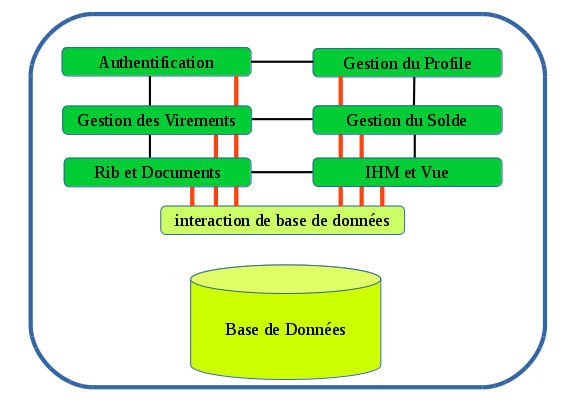
\includegraphics[width=1\textwidth]{monopolitique.png}
                \caption{Exemple d'application de banque \textcolor{red}{Architectures Monolithique}}
            \end{center}
        \end{figure}
        \column{.5\textwidth}
        \begin{itemize}
            \item Une seule application
            \item Une seule application
            \item Une seule application
            \item Une seule application
        \end{itemize} 
    \end{columns}

                %\includegraphics[width=0.5\textwidth]{imonopolitique.pn}
\end{frame}

\section{Les architectures des Microservices}
% Placing a * after \section means it will not show in the
% outline or table of contents.
\subsection*{Principe}
    \begin{columns}
        \column{0.6\textwidth}
        \begin{figure}
            \begin{center}
            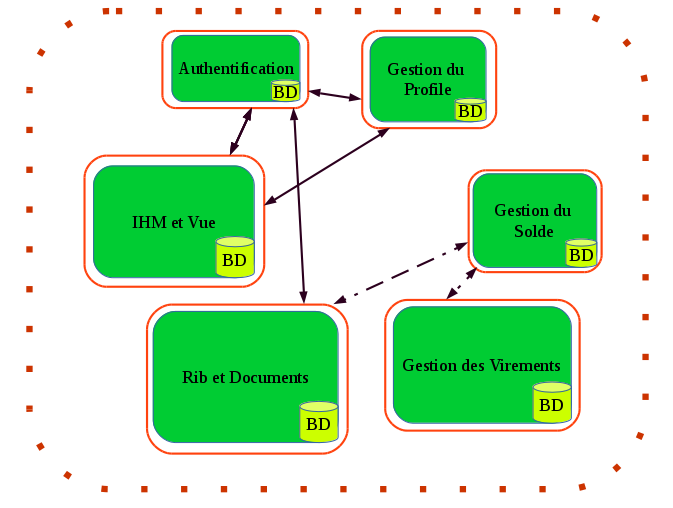
\includegraphics[width=1\textwidth]{Microservices.png}
                \caption{Exemple d'application de banque \textcolor{red}{Architectures Microservices}}
            \end{center}
        \end{figure}
        \column{.5\textwidth}
        \begin{itemize}
            \item Une seule application
            \item Une seule application
            \item Une seule application
            \item Une seule application
        \end{itemize} 
    \end{columns}

\subsection*{Isolation des Microservices}

\begin{frame}
\begin{itemize}
         \item Des services ind\'ependants
         \item Des services Isoler
\end{itemize}
\end{frame}
\subsection*{Machines virtuelles VS conteneurs }
\subsection*{Communication entre les Microservices}

\section{Avantage des Microservices }
\subsection*{D\'eploiement }
\subsection*{Mises \'a jour}
\subsection*{Bugs d\'ecentralis\'ee}
\subsection*{Scalabilit\`e}


\section{Inconv\`enients (Limites) des architectures Microservices.}

\subsection*{Taille des services}
\subsection*{Système de supervision}


\section{Conclusion}

\end{document}



